% Supplementary material: inventory figures referred to from Section 3 of the main text.

\section{Inventory Figures}
\label{supp:figures}

The figures below are generated from version~3.6 of the released inventory (releases through 4~September 2026) and are referred to from Section~\ref{sec:taxonomy} of the main text. Unless stated otherwise, they cover the 209 inventory records, that is, the 179 \glspl{slm} and the 30 small-active-parameter \glspl{moe}. Figure~\ref{fig:releases_by_size} gives releases by size band, Figure~\ref{fig:family_size_range} the size span of the principal families, Figure~\ref{fig:context_by_year} context length by year, Figure~\ref{fig:moe_vs_dense} the dense and \gls{moe} split, and Figure~\ref{fig:modality} supported modalities.

\begin{figure}[t]
  \centering
  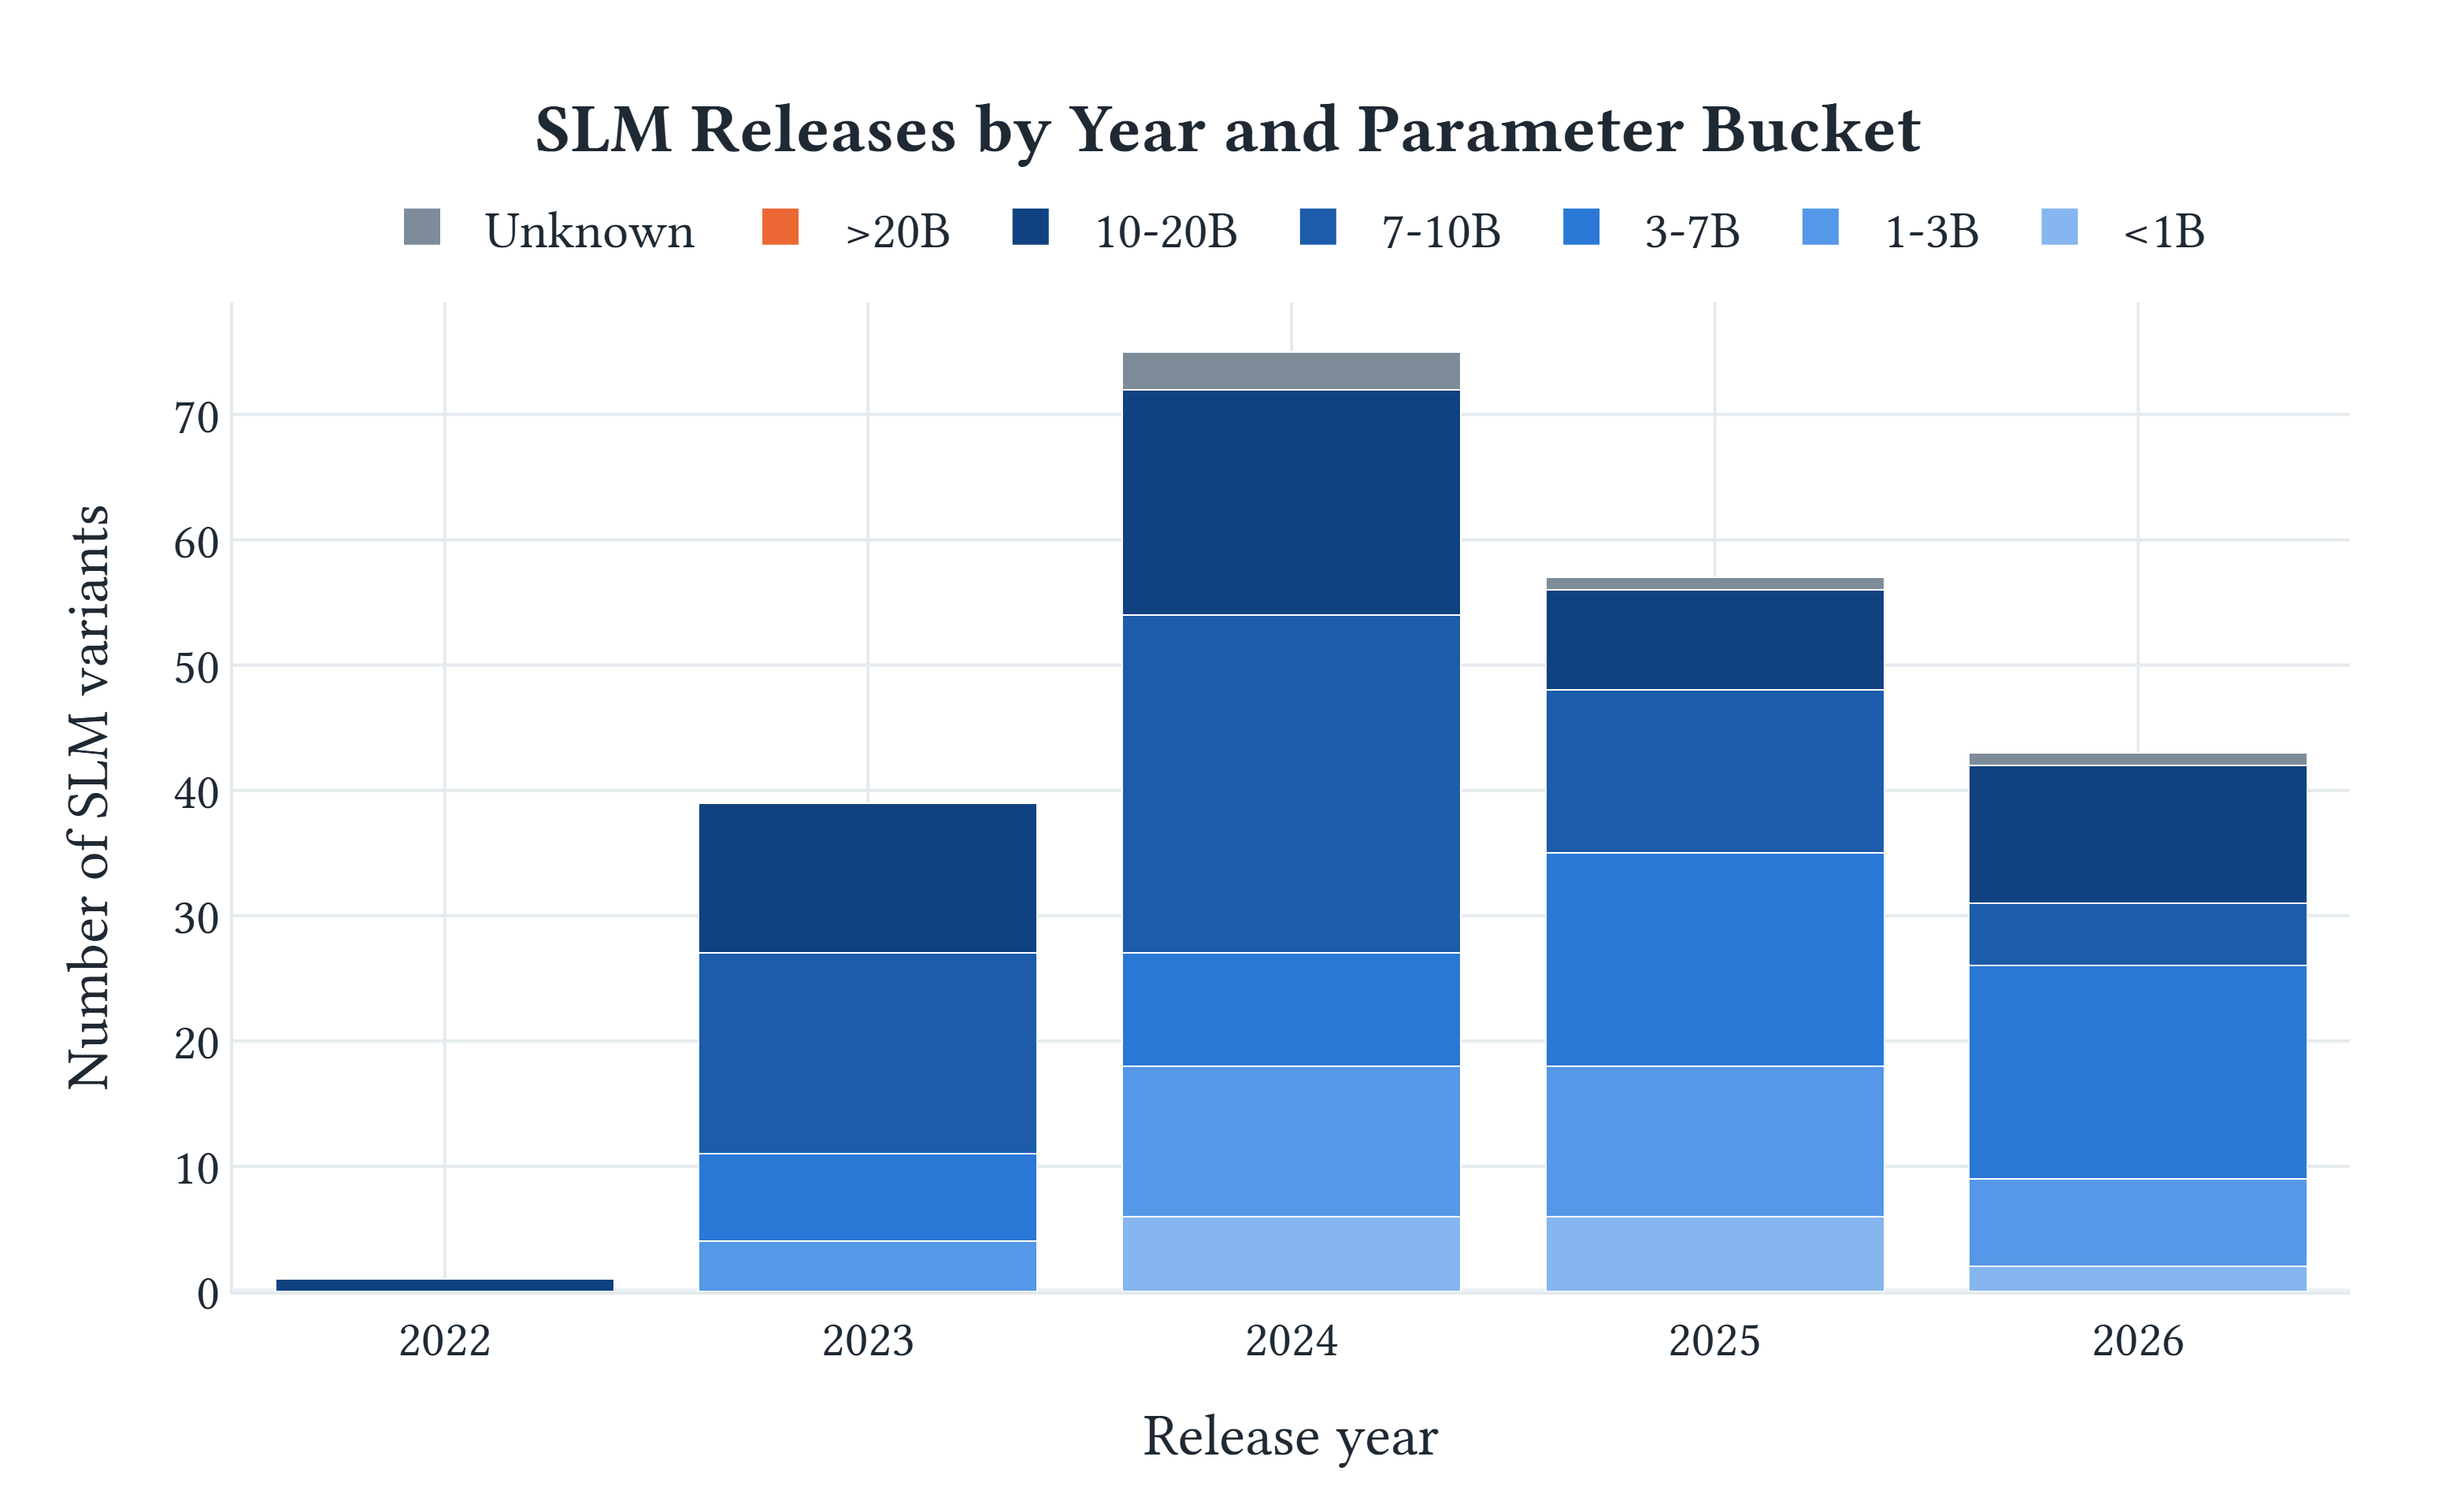
\includegraphics[width=\linewidth]{paper_slm_releases_by_size.png}
  \caption{Inventory variants by release year and total-parameter band (2026 to 4~September). The 7--10B band is the largest in 2023, 2024, and 2025; the sub-1B and 1--3B bands appear in numbers from 2024; in 2026 the largest band is the one above 20B total, which consists of small-active-parameter MoEs.}
  \Description{Stacked bar chart of inventory releases per year, split by total-parameter band. The 7-10B band is the largest from 2023 to 2025; sub-1B and 1-3B releases appear in numbers from 2024; in 2026 the band above 20B total parameters, made up of small-active-parameter mixtures of experts, is the largest.}
  \label{fig:releases_by_size}
\end{figure}

\begin{figure}[t]
  \centering
  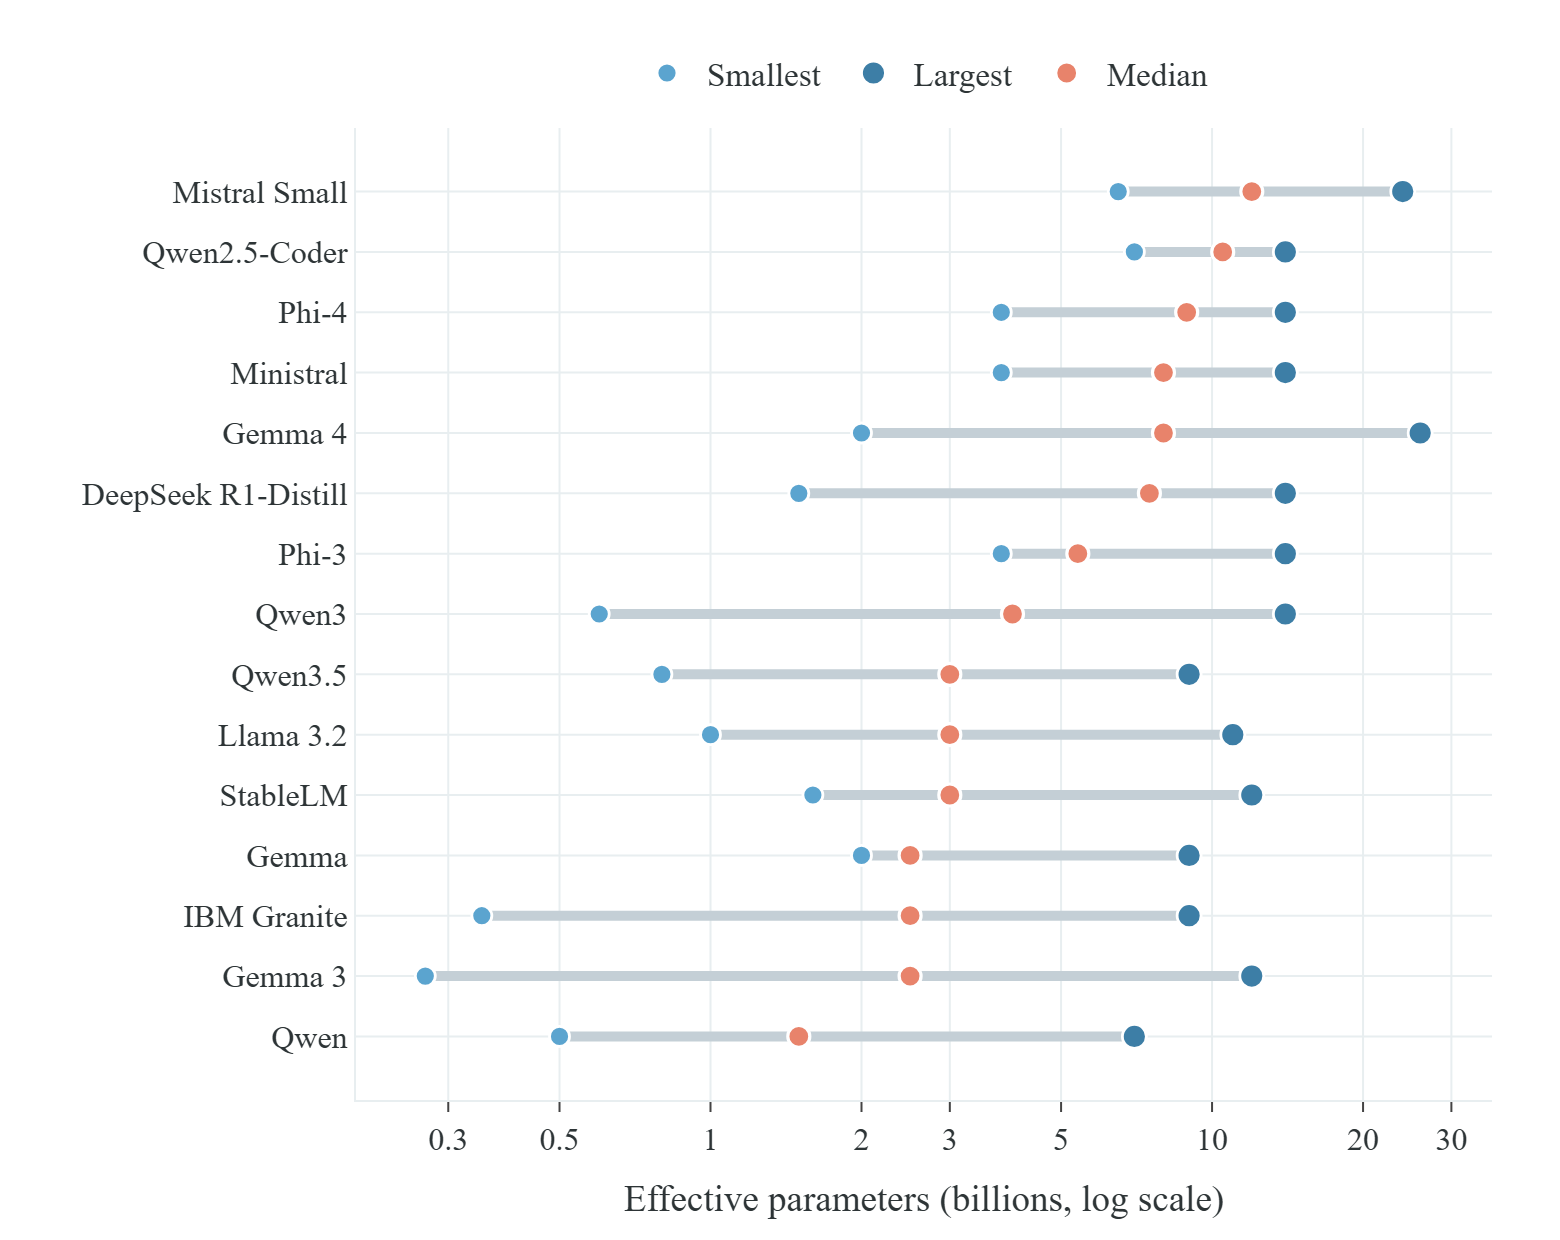
\includegraphics[width=\linewidth]{paper_slm_family_size_range.png}
  \caption{Parameter span (minimum, median, maximum, in billions, log scale) of the principal families in the inventory.}
  \Description{Horizontal range plot on a logarithmic axis showing the minimum, median, and maximum parameter count in billions for each principal family.}
  \label{fig:family_size_range}
\end{figure}

\begin{figure}[t]
  \centering
  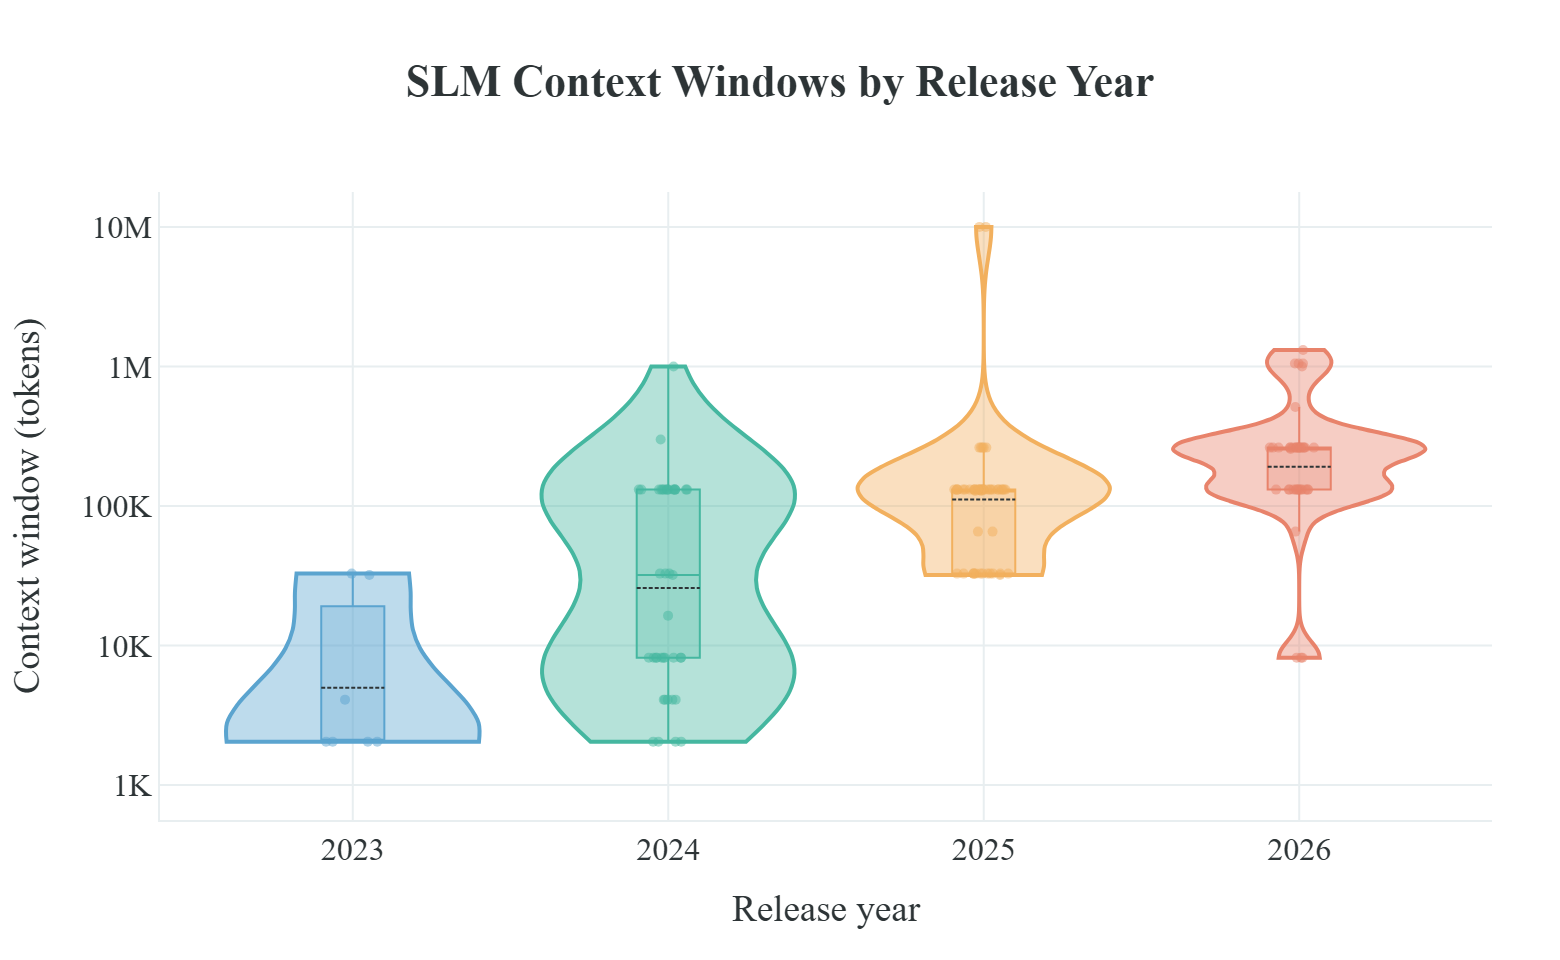
\includegraphics[width=\linewidth]{paper_slm_context_by_year.png}
  \caption{Supported context window of inventory variants by release year (log scale), for the records that state one: 5 of 36 in 2023, 39 of 74 in 2024, 52 of 58 in 2025, and 39 of 41 in 2026. Each violin is a kernel-density estimate; the inner box marks the interquartile range, the dashed line the mean, and the dots individual models. Because 2023 coverage is thin and 2026 includes small-active-parameter MoEs, the trend is indicative.}
  \Description{Violin plot of supported context window on a logarithmic axis against release year. The distribution shifts upward from a few thousand tokens in 2023 to a median of about one hundred thousand tokens or more from 2025.}
  \label{fig:context_by_year}
\end{figure}

\begin{figure}[t]
  \centering
  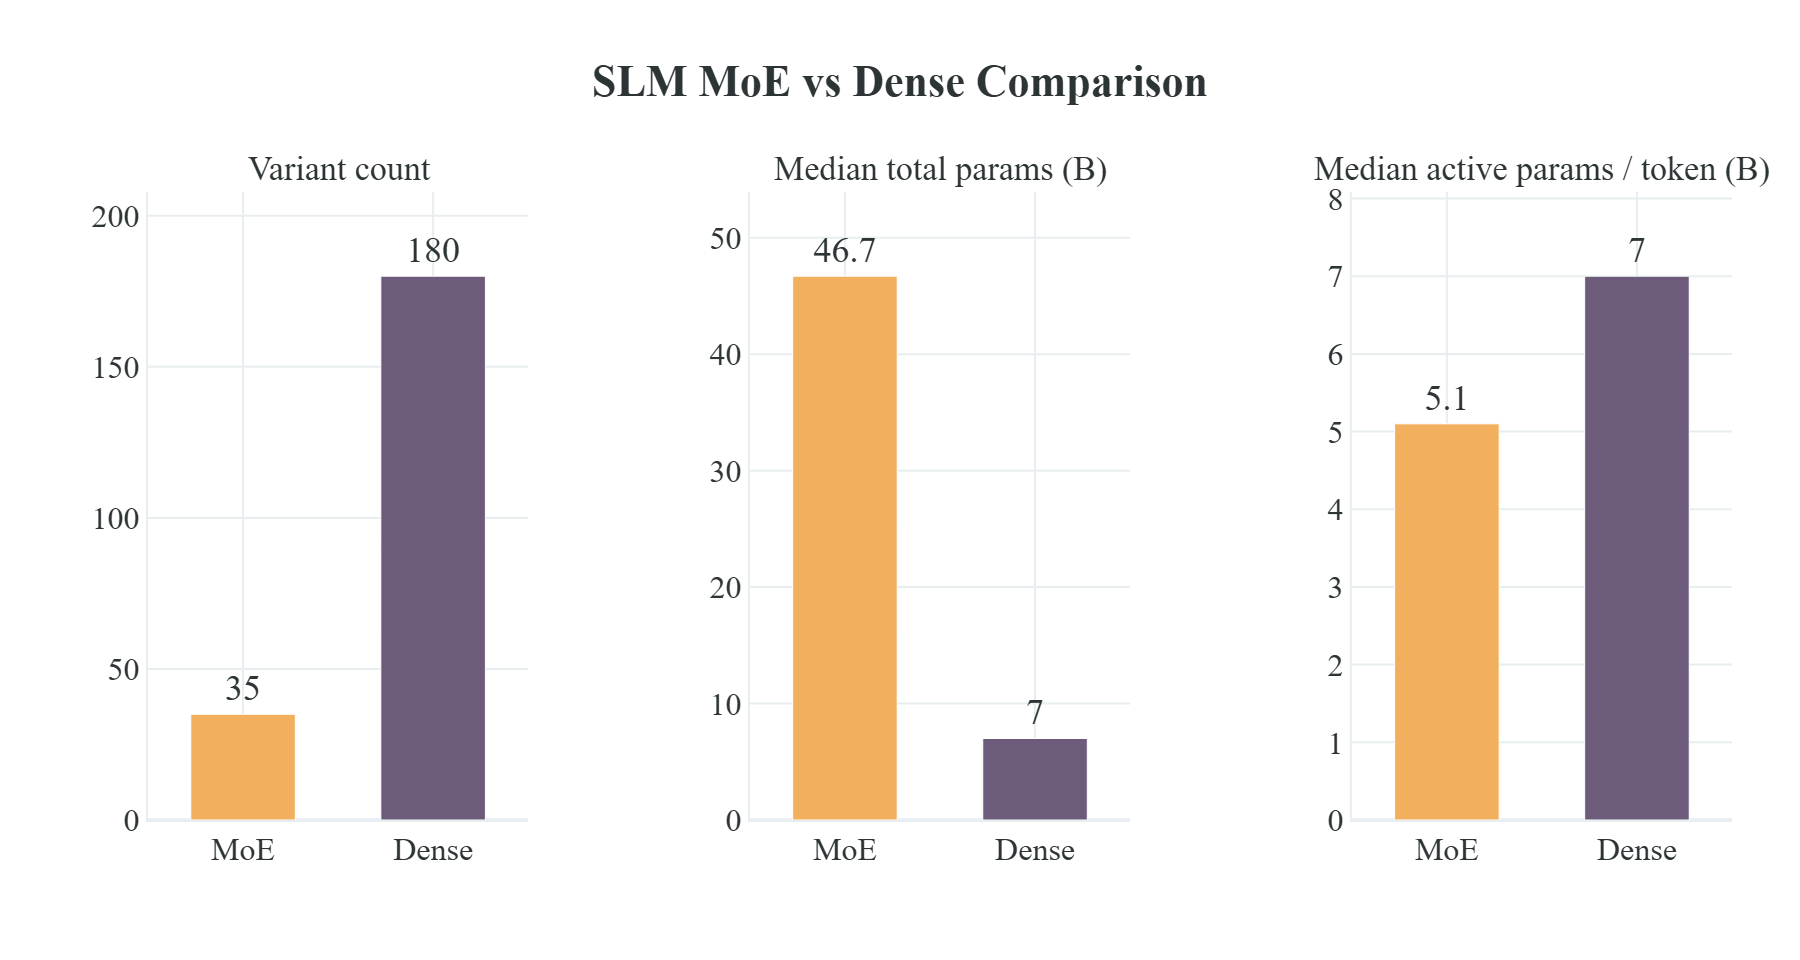
\includegraphics[width=\linewidth]{paper_slm_moe_vs_dense.png}
  \caption{Mixture-of-experts versus dense variants in the inventory: variant count (left), median total parameters (centre), and median \emph{active} parameters per token (right). MoE models carry a much larger total parameter count at a per-token cost comparable to dense models, which is the distinction between conditions C1 and C2.}
  \Description{Three side-by-side bar charts comparing mixture-of-experts and dense variants on count, median total parameters, and median active parameters per token. Dense models are far more numerous; mixture-of-experts models carry much larger totals at comparable active counts.}
  \label{fig:moe_vs_dense}
\end{figure}

\begin{figure}[t]
  \centering
  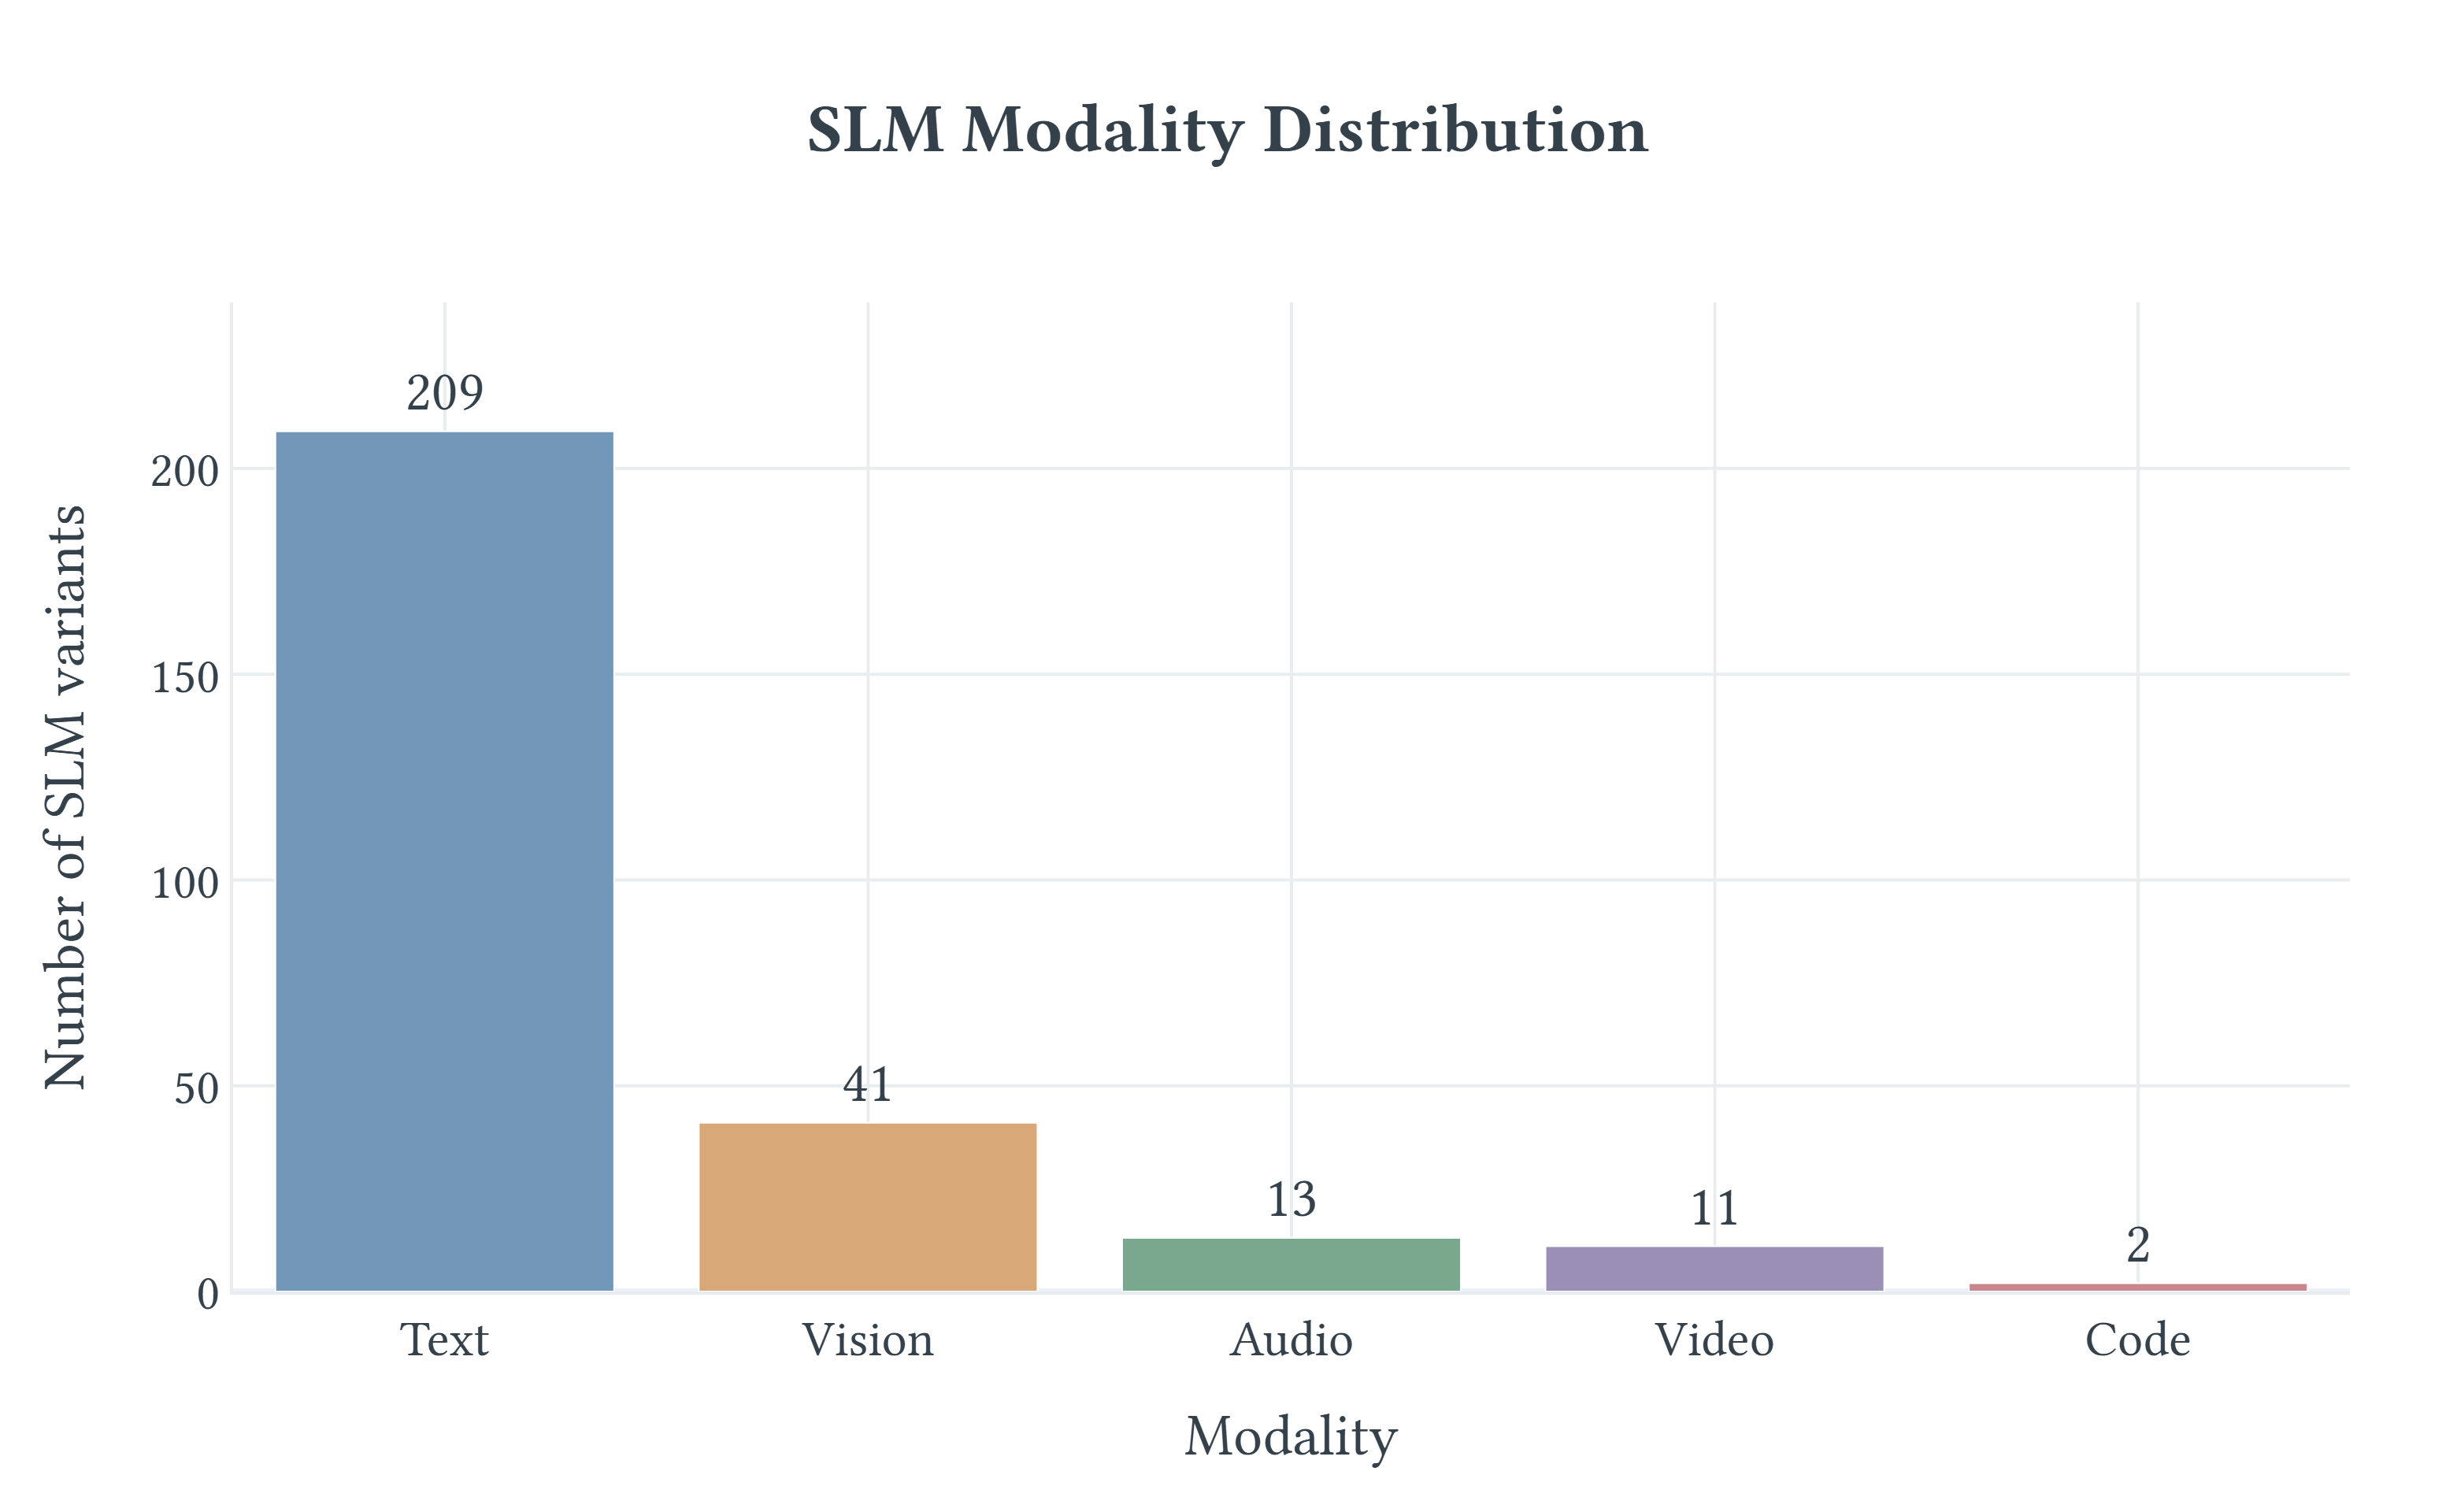
\includegraphics[width=\linewidth]{paper_slm_modality_distribution.png}
  \caption{Input modalities supported by inventory variants (a variant may support several). Text dominates, vision is common, and audio and video remain a small minority.}
  \Description{Bar chart of the number of inventory variants supporting each input modality. Text dominates, vision is common, and audio and video are small categories.}
  \label{fig:modality}
\end{figure}
